\subsection{Bestehende Konzepte und zukünftige Flugzeugmodelle}
In diesem Teil ist beschrieben, welche Flugzeugmodelle und -konfigurationen mit beschriebenen im Teil \ref{s:Neartige Antribe} Antrieben
sind in näheren Zukunft zu erwarten. Vor allem sind hier die Modelle ohne hybride Nutzung den fossilen Energieträger zusammengefasst.

Aufgrund ihrer Drop-In Fähigkeit werden die SAFs keine neuen Luftfahrzeugkonfigurationen brauchen. Was als Vorteil für den SAF betrachtet werden kann,
angesichts der aktuell produzierten Flugzeuge, die mindestens 20 Jahr im Einsatz sein werden (Quelle).
Die Abbildung stellt Eintrittsjahren für alternative Antriebe dar.
%
\begin{figure}[h]
	\centering
	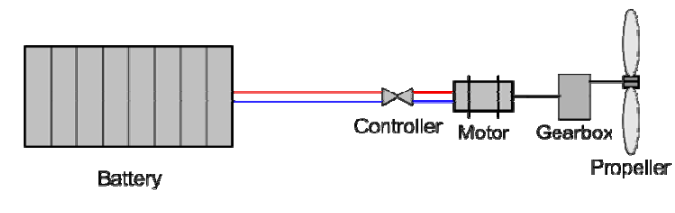
\includegraphics[width=0.9\linewidth]{Bilder/BA.png}
	\caption[Einfaches Modell eines Batterieantriebs]{fdd}
	\label{eis_antriebe}
\end{figure}
%
Positive Auswirkungen auf die Emission-Werte können bereits mit bestimmten Flugzeug- und Triebwerkskonfigurationen erreicht werden.
Zum Beispiel "Claire Liners" vom Bauhaus Luftfahrt e. V. München nicht nur aerodynamische Vorteile mitbringt, 
sondern auch Verringerung des Kraftstoffverbrauchs und damit Reduktion der Emissionen.
Jedoch sind mehr Änderungen notwendig, um netto null \cite{CO2}-Werte zu erreichen.
Die Herstellung bereitet Schwierigkeiten, manchen Firmen müssen den Geschäftsbetrieb einstellen, wie Universal Hydrogen.
\\
\textbf{Konfigurationen mit Batterie-Antrieb}\\
Wie bereits erwähnt wurde, haben die zurzeit bestehenden Batterien die geringe Energiedichte. Dadurch es ist zu erwarten, dass bis zum Jahr 
2050 keine große vollelektrische Flugzeuge hergestellt werden, sondern werden die Regional- und Kurzstrecken in den Mittelpunkt gestellt.

ES-19\\
Ein vielversprechender Prototyp war die ES-19 von Heart Aerospace. Das Unternehmen versprach die Beförderung von 19 Passagiere über 400 km mit einem BA. 
Das Flugzeug war für die Regionalstrecken konzipiert und somit konnte die geringe Nachfrage gedeckt werden. 
Außerdem waren geringe Betriebs- und Wartungskosten erwartet (Quelle).
Jedoch zu dem Zeitpunkt wurde das Flugzeug auf ES-30 mit einem hybriden Antrieb umgerüstet.


\textbf{Konfigurationen mit Wasserstoff-Antrieb}

Embraer zeigte eine Reihe von nachhaltigen Flugzeugen \textit{ENERGIA}. Die Flugzeuge sind mit unterschiedlichen Antriebe ausgestattet, unter anderem 
hybrid-elektrisch, Wasserbrennstoffzelle und Wasserstoffturbine. Bei Wasserstoffturbine wurde das Konzept von Dualen-Treibstoff vorgeschlagen, 
wo entweder Jet-A/SAF oder Wasserstoff benutzt werden kann. Das Unternehmen spricht über Technologiebereitschaft ab dem Jahr 2030, Wasserstoffturbine
ab Jahr 2035 und Wasserstoffturbine bei dem Jahr 2040. \cite{embraer_energia_2021}
%
Airbus \cite{airbus_zea_concepts} hat im Jahr 2020 drei unterschiedlichen emissionsfrei \textit{ZEROe} Konzepte vorgestellt: Turbofan, Turboprop 
und ein mit „Blended-wing body“-Design.
In allen Konzepten ist der Wasserstoff im Einsatz und Antrieb mit Gasturbinentriebwerk. Die Reichweite breitet sich ab über 1.850 - 
3700 km und die Anzahl beförderte Passagiere wird von 100 bis 200 geschätzt. Das Unternehmen will die Technologien bis zum 2035 zur Einsatzreife bringen.

Wright Spirit \cite{wright_electric_website} hat ein Konzept auf der Basis der konventionellen Flugzeug BAe 146 vorgestellt, aber mit einem Wasserstoff-Antrieb.
Das Flugzeug soll mit 4 Triebwerken, 2,5 MW Motoren und vorgestellter Batterie mit 800 Wh/kg eine Reichweite von 1000 
km erreichen und 100 Passagiere transportieren.


Universal Hydrogen

ZeroAvia stellt ihrer hybrid Wasserstoff-elektrischen Antriebe mit 3 unterschiedlichen Leistungen und Kapazitäten vor. Das kleinste davon
ist Antrieb ZA600 mit einer Leistung von 600 kW, mit der Möglichkeit bis 20 Passagieren über 555 km zu befördern. 
Geplante Eintrittzeit (Entry-in-System EIS) ist im Jahr 2025. Der Antrieb ist mit gasförmigem Wasserstoff angetrieben.
%Flugzeug mit 80 Menschen verbraucht bis zu 80% weniger Treibstoff pro STD/kg (5 mal weniger)

Es wurden eine Menge kleineren elektrischen Flugzeugen vorgestellt, die manche wurden sogar erprobt.
Institut für Flugzeugbau am Universität Stuttgart entwickelte ein zweisitziges hybrid-batteriebetriebenen Segelflugzeug \textit{e-Genius}. Das Flugzeug soll
die Reichweite von 400 km erreichen und hat die Batteriekapazität von 40 kWh mit 1,5 Stunden Ladedauer. %Quelle https://www.ifb.uni-stuttgart.de/en/research/mannedaircraft/e-genius/
Pipistrel  Alpha Electro hat bereits im Jahr 2007 sein erstes elektrischen Zweisitzer vorgestellt, mittlerweile das Modell "Velis Electro" wird
für das Pilottraining mit einem Triebwerk mit 57.6 kW Leistung. Der Antrieb ist flüssigkeitsgekühlt und braucht ein externes Ladegerät.
%https://www.pipistrel-aircraft.com/products/velis-electro/


Es werden unterschiedliche wasserstoffkonfugurationen vorgeschlagen aufgrund des schweren und massiven Wasserstofftanks.
Es gibt Konzepte, wo der Tank am Rumpf, am Ende des Rumpfes, vorne hinter Pilotenkabine
Wie ist zu sehen, es werden viele Konzepte zurzeit ausgearbeitet. Es lässt sich abwarten bis Technologien tatsächlich auf den Markt kommen.